%% LyX 1.1 created this file.  For more info, see http://www.lyx.org/.
%% Do not edit unless you really know what you are doing.
\documentclass[10pt,oneside,english,british]{book}
\usepackage{times}
\usepackage[T1]{fontenc}
\usepackage[latin1]{inputenc}
\usepackage{a4wide}
\usepackage{fancyhdr}
\pagestyle{fancy}
\usepackage{babel}
\setcounter{secnumdepth}{3}
\setcounter{tocdepth}{3}
\setlength\parskip{\smallskipamount}
\setlength\parindent{0pt}
\usepackage{graphics}

\makeatletter

%%%%%%%%%%%%%%%%%%%%%%%%%%%%%% LyX specific LaTeX commands.
\providecommand{\LyX}{L\kern-.1667em\lower.25em\hbox{Y}\kern-.125emX\@}

%%%%%%%%%%%%%%%%%%%%%%%%%%%%%% User specified LaTeX commands.
\renewcommand{\headrulewidth}{0.4pt}
\renewcommand{\footrulewidth}{0.4pt}
\lhead{\resizebox{1in}{!}{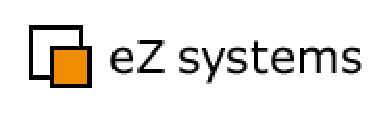
\includegraphics{screenshots/2.0/ezsystems.eps}}}
\rhead{}
\chead{}

\makeatother
\AtBeginDocument{
  \renewcommand{\labelitemiv}{}
}

\begin{document}

\title{eZ publish Installation Guide}


\author{\resizebox*{0.75\columnwidth}{!}{
\includegraphics{screenshots/2.0/ezpublish.eps}} }

\maketitle
\resizebox*{!}{0.2in}{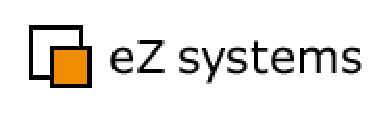
\includegraphics{screenshots/2.0/ezsystems.eps}} The
double squares and eZ are trademarks belonging to eZ systems of Norway,
registration number NO 981 601 564 (http://www.brreg.no/oppslag/enhet/detalj.ssc?orgnr=981601564).

All images and text herein is Copyright 2001 eZ systems.

eZ publish is a software package released under the GPL lisence (http://www.gnu.org/copyleft/gpl.html),
its primary point of distribution and information is http://developer.ez.no/

\tableofcontents{}


\chapter{Introduction\label{chptr: introduction}}

\begin{quote}
\textbf{{}``He who asks is a fool for five minutes, but he who does
not ask remains a fool forever.{}''} - \-
\end{quote}
eZ publish is a content management system, among a lot of other things.
This installation manual will try to cover the job of installing eZ
publish on your server.

This manual covers installation on a Red Hat Linux system; most of
what is described here can also be applied to other installations,
especially if your system uses RPM for installation. For other systems
you would need to do a lot of compiling yourself to make this work,
or apply the system's own package manager.

Finding packages can be done dirctly from vendor sites, though you
might not be guaranteed that you'll find the package you need. In
such instances you need to download the source directly from the software
developer.

Different distribution sites for different Unix systems are:

\begin{itemize}
\item Debian \texttt{\footnotesize (http://www.debian.org/distrib/ftplist)}{\footnotesize \par}
\item Mandrake, see chapter \ref{chptr: mandrake}.
\item IRIX \texttt{\footnotesize (http://freeware.sgi.com/)}{\footnotesize \par}
\item Red Hat Linux \texttt{\footnotesize (http://www.redhat.com/apps/download})
\item SuSE Linux (\texttt{\footnotesize http://www.suse.com/us/support/download/index.html)}{\footnotesize \par}
\item Sun \texttt{\footnotesize (http://www.sunfreeware.com/)}{\footnotesize \par}
\end{itemize}
The addresses to the software developers will be given where apropriate
in the text.

You can also try \char`\"{}The Written Word\char`\"{} (\texttt{\footnotesize ftp://ftp.thewrittenword.com/packages/free/by-name/gcc-2.95.2/})
for binaries for Solaris 2.5.1, 2.6, 2.7/SPARC, 2.7/Intel, IRIX 6.2,
6.5, Digital UNIX 4.0D, HP-UX 10.20, and HP-UX.


\section{Pre-Configured Hosting}

It is possible to get pre-configured hosting services where you can
install and manage your eZ publish site with ease. Read more about
our hosting partners at eZ systems web site (\texttt{\footnotesize http://en.ez.no/article/articlestatic/73}).


\section{Pre-Configured Hardware}

It is possible to order pre-configured hardware from eZ systems. You
can order through or web shop (\texttt{\footnotesize http://sourceprovider.com/}).

A line starting with a hash-sign {}``\#{}'' are input from the user
to the shell.


\chapter{Pre-requisites\label{chptr: pre-requisites}}


\section{Needed Privileges}

For the standard installation (and for the moment the only method)
of eZ publish you will need to have the following privileges on your
system:

\begin{itemize}
\item Access to Apache's httpd.conf
\item Access to compiler (You will have to install the gcc compiler on your
system, see chapter \ref{chptr: introduction} for a list of sites
providing software for different Unixes.)
\item Access to a shell (You must run certain scripts during installation.
Some of them are just creating links to different directories; you
might therefore just create those links via FTP.)
\item Access to a shell
\item Access to cron jobs (Only needed if you want to use the eZ news feed
module for regular updates of headlines imported from other sites.)
\item Access to Apache's modules
\item Access to a MySQL database
\item You might also need the privilege to add new libraries to your system.
\end{itemize}
You might also use other web servers than apache, but then you're
on your own since we haven't tested eZ publish on other configurations.
If you do try another web server, please keep a log of what you do
and submit it to us (pkej@ez.no) for inclusion in future versions
of this manual.


\section{Needed Software}

You also need to download and install the following packages, if they
aren't present on your system already:

\begin{itemize}
\item MySQL (http://www.mysql.com) version 3.23 or later. (eZ publish requires
MySQL for storage of its data.)
\item libXml (http://xmlsoft.org/\#Downloads) version 2.2.7, 2.2.8 or 2.2.9.
(Needed by eZ article. If you wish to use the default article renderer
you need libXml2 installed. You can create your own renderers if you
don't want to use the default.)
\item libQdom (http://www.trolltech.com) is a part of QT, you need version
2.2.3 or later. (Needed by eZ news feed's parsers. If you wish to
include headlines from external sites (example developer.ez.no or
slashdot.org) then you need this installed. You can create your own
parsers if you don't want to use the default.)
\item ImageMagick (http://www.imagemagick.org/) newest version (Needed by
eZ article, eZ image catalogue, and all modules using images. You
need only the command line version.)
\item Apache (http://httpd.apache.org/) latest 1.3 release. (It is always
recommended to run the latest Apache release, though eZ publish shouldn't
be very picky with the Apache versions. We've used eZ publish with
Apache 1.3.13, some have reported that Apache 1.3.9 isn't useful.)
\item Any and all modules you need for apache in addition to mod\_php. (http://modules.apache.org/)
\item PHP (http://www.php.net/) version 4.0.4pl1 or later, you need the
source code version. (eZ publish uses references for objects and foreach
loops. Only version 4.0.4pl1 and later supports both of these features
satisfactorily.)
\item eZ publish (http://developer.ez.no/) verision 2.0 or later stable
releases.
\end{itemize}
The libraries and php will appear pre-compiled for Linux i386 on http://developer.ez.no
in the future. The software is listed in the order of installation.


\section{Which Software is Already Installed?}


\subsection{Systems Using RPM}

RPM is a system for distributing pre-compiled software. The packages
also contain pre-configured settings and initialisation files, leaving
almost nothing to the user, except deciding what to install.

To check if a package is available on your system you can run the
following command (RPM based systems {}``rpm -qa | grep <name of
program/library>{}''. If you need to know where you can find the
different files from that package you can follow up on the previous
command with the following {}``rpm -ql <rpm name>{}''. RPM name
is one of the returned names from the previous command, example:\\


\texttt{\footnotesize ~~~~\# pkej@vogol:/etc/httpd > rpm -qa |
grep libxml}{\footnotesize \par}

\texttt{\footnotesize ~~~~libxml-1.8.7-80}{\footnotesize \par}

\texttt{\footnotesize ~~~~libxmld-1.8.7-80}{\footnotesize \par}

\texttt{\footnotesize ~~~~\# pkej@vogol:/etc/httpd > rpm -ql libxml-1.8.7-80}{\footnotesize \par}

\texttt{\footnotesize ~~~~/usr/bin/xml-config}{\footnotesize \par}

\texttt{\footnotesize ~~~~/usr/lib/libxml.so.1}{\footnotesize \par}

\texttt{\footnotesize ~~~~/usr/lib/libxml.so.1.8.7}{\footnotesize \par}

\texttt{\footnotesize ~~~~/usr/share/doc/packages/libxml}{\footnotesize \par}

\texttt{\footnotesize ~~~~/usr/share/doc/packages/libxml/AUTHORS}{\footnotesize \par}

\texttt{\footnotesize ~~~~/usr/share/doc/packages/libxml/COPYING}{\footnotesize \par}

\texttt{\footnotesize ~~~~/usr/share/doc/packages/libxml/COPYING.LIB}{\footnotesize \par}

\texttt{\footnotesize ~~~~/usr/share/doc/packages/libxml/NEWS}{\footnotesize \par}

\texttt{\footnotesize ~~~~/usr/share/doc/packages/libxml/README}{\footnotesize \par}

\texttt{\footnotesize ~~~~/usr/share/doc/packages/libxml/TODO}{\footnotesize \par}


\section{FreeBSD}

When installing and compiling PHP on a FreeBSD system you might encounter
an error when using --with-dom which says you have a conifgure error
on the lib. It turns out that the current port of libxml installs
itself as /usr/local/lib/libxml2.a|so and it goes unrecognised by
configure. You can easily get around this problem by linking the libs
to libxml.a|so.


\section{Mandrake}

First read chapter \ref{chptr: mandrake}, then continue reading the
manual from here.


\section{IRIX}

By accessing the software manager (you must be root) you can get a
list of installed software, scroll or search that list to find the
packages you're interested in. Double click on the tabs to the left
to get information about where specific files are installed.


\section{RAQ 3}

There is a separate chapter \ref{chptr: raq 3} in this manual describing
installation on a RAQ 3 server. It was kindly provided by Chris Mason, 


\section{Windows}

Windows installation is described in its own chapter \ref{chptr: windows}.


\section{Other Systems}

On other systems you should read the documentation for that system
to learn how to find out what software is already installed.

You could try to use the command {}``find{}'' to find the software.
It is used thus: {}``find . -name \textbackslash{}{*}<program name>\textbackslash{}{*}{}''
from the /usr/, /local/ , /lib/, /share/ directories. In extreme cases
you could try from the root of the system, but this will take a long
time and will also hog resources on your computer. Therefore we urge
you to learn how to use the proper installation features of your system
to find the software already installed.


\section{Installation of Required Software}

If you've found pre-compiled versions of all the software packaged
for use with an installation tool, you just have to install that software
using the tool. Instructioins for its usage is often found using the
command {}``man <installation tool name>{}'' or by reading your
system's documentation or the supplier's website.

If you've had to download source code you will find instructions on
how to compile and install the software you've downloaded at the software
developer's website. This requires a bit of knowledge and you should
only undertake this if you feel confident about the job.

This manual will only cover configuration of the software needed and
compilation of PHP to use the other software.


\section{Important Notice}

You should read all the README, INSTALL and similar files found with
the software packages you download. They often contain tips on how
to configure, compile and install the software on your system. It
will save you a lot of time and aggravation if you follow instructions
supplied with the software.

If problems arise during installation of the software, please turn
to the suppliers support forums, mailing list archives and FAQs, your
questions will often be answered there. If the supplier's forums doesn't
seem to help you, you should check the support forums at our site.

You should always do a search of the forums before posting any questions.


\chapter{Compile Configuration}


\section{PHP}


\subsection{Unpacking}

After you have downloaded PHP you need to unpack it somewhere where
you can compile and configure the software. To unpack run the command:\\


\texttt{\footnotesize ~~~~\# tar zxvf php-4.0.x.tar.gz}~\\
{\footnotesize \par}

Where the x is the version of php you've downloaded. Then you need
to move into the directory you extracted php into:\\


\texttt{\footnotesize ~~~~\# cd php-4.0.x}{\footnotesize \par}


\subsection{Configuration}

You'll need either an apache module or a command line version of PHP
to use eZ publish on your website. We recommend you use PHP as an
apache module. You will also need the command line version if you
want to use the cron jobs for periodical updates of the eZ news feed
module.

Thus for our recommended installation of PHP you need both the command
line and module versions of PHP.


\subsubsection{Common}

Both the command line and apache module versions need to have the
following configurations added to the configuration tool:

\begin{description}
\item [--enable-trans-sid]This lets PHP use session id's which don't rely
on cookies. It does not disable normal cookie based sessions.\\
({\footnotesize http://www.php.net/manual/en/install.configure.php\#install.configure.enable-trans-sid})
\item [--with-mysql]This tells PHP that the mysql functionality should be
used.\\
({\footnotesize http://www.php.net/manual/en/install.configure.php\#install.configure.with-mysql})
\item [--enable-magic-quotes]This tells PHP to enable magic quotes by default.
you can also turn this feature on and off on a directory by directory
basis in either the {}``.htaccess{}'' files (if you use them) or
in the setup of the virtual server in {}``httpd.conf{}''.\\
({\footnotesize http://www.php.net/manual/en/install.configure.php\#install.configure.enable-magic-quotes})
\item [--with-dom]This configures PHP to include libxml. {\footnotesize }\\
{\footnotesize (http://www.php.net/manual/en/install.configure.php\#install.configure.with-dom)}{\footnotesize \par}
\item [--with-qtdom]This configures PHP to include libqdom. It isn't up
on the PHP site with a link, but it works as --with-dom.
\end{description}
You should also go through the web page: {\footnotesize http://www.php.net/manual/en/install.configure.php}
and make sure that there isn't other functionality you would like
to have included.


\subsubsection{Command Line}

The default is to create a command line version of PHP. Therefore
you don't need to add more configuration options for this.


\subsubsection{Apache Module}

To build an apache module you need to add:

\begin{description}
\item [--with-apxs]This compiles PHP as an apache module. {\footnotesize }\\
{\footnotesize (http://www.php.net/manual/en/install.configure.php\#install.configure.with-apxs)}{\footnotesize \par}
\end{description}

\subsubsection{Other Web Servers}

We haven't tested our software with other web servers than apache.
If you need to try out other web servers, read this document {\footnotesize http://www.php.net/manual/en/install.configure.php\#install.configure.servers}
to learn how you configure for the web server you will be using.


\subsubsection{Creating the Configuration}

Now you just have to run the {}``./configure{}'' program with the
apropriate configuration directives which we discussed in the preceeding
sections, for an apache module you'd do the following:\\


\texttt{\footnotesize ~~~\# ./configure -{}-enable-trans-sid -{}-with-mysql
-{}-with-magic-quotes}~\\
\texttt{\footnotesize ~~~~-{}-with-apxs} {\selectlanguage{english}}\texttt{\footnotesize -{}-with-dom
-{}-with-qtdom}~\\
{\footnotesize \par}

Remember that to compile a script/cgi version you'd need to change
that line to:\\


\texttt{\footnotesize ~~~~\# ./configure -{}-enable-trans-sid
-{}-with-mysql -{}-with-magic-quotes}~\\
\texttt{\footnotesize ~~~~-{}-with-dom -{}-with-qtdom}{\footnotesize \par}


\subsection{Compilation}

To compile you need to run the command {}``make{}'':\\


\texttt{\footnotesize ~~~~\# make}{\footnotesize \par}


\subsection{Installation}

To install your new PHP package you need to run the following command:\\


\texttt{\footnotesize ~~~~\# make install}{\footnotesize \par}


\chapter{Apache Configuration}

For the moment we have only one solution for configuring apache, and
that is using two virtual hosts.


\section{Dual Virtual Host}


\subsection{Configuring Through httpd.conf}

This set up is based on having two different virtual hosts for your
administration back-end and the main site. The main site would typically
be known as {}``www.yoursite.com{}'' and the administration would
be {}``admin.yoursite.com{}''; the names are up to you, theoretically
you could have different names, for example {}``mysite.yoursite.com{}''
and {}``administration.mysite.com{}''.

The virtual host is configured through the {}``httpd.conf{}'' file
which is the main configuration of Apache. Following is an example
of such a host, remember to exchange everything within brackets ({}``{[}{}``
and {}``{]}{}'') with your preferred and local settings and also
remove the brackets.


\subsubsection{User Site}

\texttt{\scriptsize ~~~~\# User site}{\scriptsize \par}

\texttt{\scriptsize ~~~~<VirtualHost~{[}your.domain.com{]}>}{\scriptsize \par}

\texttt{\scriptsize ~~~~~~<Directory~{[}/your/apache/documentroot/publish\_dist{]}>}{\scriptsize \par}

\texttt{\scriptsize ~~~~~~~~Options~FollowSymLinks~Indexes~ExecCGI}{\scriptsize \par}

\texttt{\scriptsize ~~~~~~~~AllowOverride None}{\scriptsize \par}

\texttt{\scriptsize ~~~~~~</Directory>}{\scriptsize \par}

\texttt{\scriptsize ~~~~~~RewriteEngine On}{\scriptsize \par}

\texttt{\scriptsize ~~~~~~RewriteRule~\textasciicircum{}/filemanager/filedownload/({[}\textasciicircum{}/{]}+)/(.{*})\$}{\scriptsize \par}

\texttt{\scriptsize ~~~~~~{[}/your/apache/documentroot{]}/publish\_dist/ezfilemanager/files/\$1}{\scriptsize \par}

\texttt{\scriptsize ~~~~~~{[}T=\char`\"{}application/oct-stream\char`\"{},S=1{]}}{\scriptsize \par}

\texttt{\scriptsize ~~~~~~\#~The~lines~above~should~appear~on~the~same}{\scriptsize \par}

\texttt{\scriptsize ~~~~~~\#~line~in~your~configuration~file!}{\scriptsize \par}

\texttt{\scriptsize ~~~~~~RewriteRule !\textbackslash{}.(gif|css|jpg|png)\$
{[}/your/apache/documentroot{]}/publish\_dist/index.php}{\scriptsize \par}

\texttt{\scriptsize ~~~~~~ServerAdmin {[}your e-mail address{]}}{\scriptsize \par}

\texttt{\scriptsize ~~~~~~DocumentRoot {[}/your/apache/documentroot{]}/publish\_dist}{\scriptsize \par}

\texttt{\scriptsize ~~~~~~ServerName {[}your.domain.com{]}}{\scriptsize \par}

\texttt{\scriptsize ~~~~~~ServerAlias publish}{\scriptsize \par}

\texttt{\scriptsize ~~~~</VirtualHost>}{\scriptsize \par}


\subsubsection{Admin Site}

\texttt{\footnotesize ~~\# Admin site }{\footnotesize \par}

\texttt{\footnotesize ~~<VirtualHost admin.yourdomain.org>}{\footnotesize \par}

\texttt{\footnotesize ~~~~<Directory {[}/your/apache/documentroot/admin{]}>}{\footnotesize \par}

\texttt{\footnotesize ~~~~~~Options FollowSymLinks Indexes ExecCGI}{\footnotesize \par}

\texttt{\footnotesize ~~~~~~AllowOverride None}{\footnotesize \par}

\texttt{\footnotesize ~~~~</Directory>}{\footnotesize \par}

\texttt{\footnotesize ~~~~RewriteEngine On}{\footnotesize \par}

\texttt{\footnotesize ~~~~RewriteRule !\textbackslash{}.(gif|css|jpg|png)\$
{[}/your/apache/documentroot/admin/index.php{]}}{\footnotesize \par}

\texttt{\footnotesize ~~~~ServerAdmin {[}your\_mail@domain.no{]}}{\footnotesize \par}

\texttt{\footnotesize ~~~~DocumentRoot {[}/your/apache/documentroot/admin{]}}{\footnotesize \par}

\texttt{\footnotesize ~~~~ServerName {[}admin.yourdomain.org{]}}{\footnotesize \par}

\texttt{\footnotesize ~~~~ServerAlias {[}admin.yourdomain.org{]}}{\footnotesize \par}

\texttt{\footnotesize ~~</VirtualHost>}~\\
{\footnotesize \par}

The format of the {}``httpd.conf{}'' file is covered at http://httpd.apache.org/docs/
for a complete understanding of the above information you'll need
to read that documentation.

The rewrite rules does the following:\\


\texttt{\footnotesize ~~~~RewriteRule \textasciicircum{}/filemanager/filedownload/({[}\textasciicircum{}/{]}+)/(.{*})\$}{\footnotesize \par}

\texttt{\footnotesize ~~~~{[}/your/apache/documentroot{]}/publish\_dist/ezfilemanager/files/\$1}{\footnotesize \par}

\texttt{\footnotesize ~~~~{[}T=\char`\"{}application/oct-stream\char`\"{},S=1{]}}~\\
{\footnotesize \par}

This says that everything served from {}``/filemanager/filedownload/{}''
should be redirected to fetch information from {}``publish\_dist/ezfilemanager/files{}''.
In other words, when people downloads a file from the filemanager,
the file is served from the directory specified in the second part.

The {}``\^{ }{}'' just after {}``RewriteRule{}'' says that evertything
which starts with this, in other words it is a start of line marker.
When working with an URL that is from the root of your site, ie. the
part from the first slash after your domain name.

The {}``\${}'' sign is used to mark the end of line, in order to
remember the full line.

The part \texttt{\scriptsize {}``{[}T=\char`\"{}application/oct-stream\char`\"{},S=1{]}{}''}
means that everything which is matched shall be of the specific mime
type ({}``application/oct-stream{}'', ie. binary download). The
{}``S=1{}'' part means that if we match this rule, we should skip
one rule ahead before trying to match again.

The next rewrite rule:\\


\texttt{\footnotesize ~~~~RewriteRule !\textbackslash{}.(gif|css|jpg|png)\$
{[}/your/apache/documentroot{]}/publish\_dist/index.php}~\\
{\footnotesize \par}

is found in both sites (admin and user). This means that every file,
except gif, css, jpg and png (and files matched against the previous
rule when in the user site) should be redirected to the file in the
second part, ie. the index.php file. The reason for this is that we
don't want anyone trying to get direct access to anything which might
be sensitive, or revealing about the site's operation.

If you didn't compile PHP with magic quotes; or other software relies
on PHP not using magic quotes you can add the following line into
each virtual host section:\\


\texttt{\footnotesize ~~~~php\_value magic\_quotes\_gpc 1}~\\
{\footnotesize \par}

\emph{NOTE: It isn't possible to use the form http://mysite.com/admin
at all; since the admin module assumes that the url {}``/{}'' is
the start of the admin pages. If you do change eZ publish code in
order to do this anyway; please send the code to bf@ez.no for future
inclusion.}


\subsection{Configuring Through .htaccess}

Instead of using httpd.conf and rewrite rules in the virtual hosts,
you can also do the rewrite rules in the .htaccess filesm directory
specific configuration files.

\emph{Note: You must set up apache to accept this. You still need
two domains for this operation!}


\subsubsection{User Site}

In your main directory (/path/to/index.php/) create a file called
\char`\"{}.htaccess\char`\"{} containing the following text:\\


\texttt{\footnotesize ~~~~Options FollowSymLinks Indexes ExecCGI}{\footnotesize \par}

\texttt{\footnotesize ~~~~RewriteEngine On}{\footnotesize \par}

\texttt{\footnotesize ~~~~RewriteRule \textasciicircum{}/filemanager/filedownload/({[}\textasciicircum{}/{]}+)/(.{*})\$}{\footnotesize \par}

\texttt{\footnotesize ~~~~/path/to/website/ezfilemanager/files/\$1}{\footnotesize \par}

\texttt{\footnotesize ~~~~{[}T=\char`\"{}application/oct-stream\char`\"{},S=1{]}}{\footnotesize \par}

\texttt{\footnotesize ~~~~\# The lines above should appear on
the same}{\footnotesize \par}

\texttt{\footnotesize ~~~~\# line in your configuration file!}{\footnotesize \par}

\texttt{\footnotesize ~~~~RewriteRule !\textbackslash{}.(gif|css|jpg|png)\$
/path/to/website/index.php}{\footnotesize \par}


\subsubsection{Admin Site}

In your admin subdomain home directory, create a file with the following
text:\\


\texttt{\footnotesize ~~~~RewriteEngine On}{\footnotesize \par}

\texttt{\footnotesize ~~~~RewriteRule !\textbackslash{}.(gif|css|jpg|png)\$
/path/to/website/admin/index.php}~\\
{\footnotesize \par}

Note the extra \char`\"{}\textbackslash{}\char`\"{} in the rewrite
rule. Its slightly different to the line used in the httpd.conf method.


\chapter{eZ publish Installation}


\section{Program Files}

The next step is to install the eZ publish package in your document
root directory. First you need to unpack the software in a temporary
directory:\\


\texttt{\footnotesize ~~~~\# cd /tmp}{\footnotesize \par}

\texttt{\footnotesize ~~~~\# tar zxvf /path/to/ezpublish-2.0.tar.gz}~\\
{\footnotesize \par}

The next step is to move the files to your document root:\\


\texttt{\footnotesize ~~~~\# mv /tmp/publish\_dist /your/apache/documentroot}~\\
{\footnotesize \par}

When all this is done you need to tell eZ publish a little about the
site you're running. You'll need to edit the {}``site.ini{}'' file
which you will find in the document root:\\


\texttt{\footnotesize ~~~~\# cd /your/apache/documentroot}{\footnotesize \par}

\texttt{\footnotesize ~~~~\# vi site.ini}~\\
{\footnotesize \par}

Instead of vi you can use your preferred text editor. You'll need
to add information about the username, hostname and password of your
database. More information on what you can do with {}``site.ini{}''
can be found in the {}``eZ publish Customisation Guide{}''.

The next important step is to run the script modfix. This script will
create symbolic links needed and set permissions.\\


\texttt{\footnotesize ~~~~\# ./modfix\_secure.sh}~\\
{\footnotesize \par}

Then you need to create cache directories:\\


\texttt{\footnotesize ~~~~\# su}~\\
\texttt{\footnotesize ~~~~\# ./cachefix\_secure.sh {[}package\_user{]}
{[}apache\_process\_group{]}}~\\
{\footnotesize \par}

Where \texttt{\footnotesize {[}package\_user{]}} is the web admin
user and \texttt{\footnotesize {[}apache\_process\_group{]}} is the
group of the running apache process.


\section{Database}


\subsection{First Time Installation}

Now you need to create a database in MySQL, the default name we use
is publish, but you can change that to whatever pleases you.\\


\texttt{\footnotesize ~~~~\# mysqladmin create publish}~\\
{\footnotesize \par}

Add a publish user in MySQL. To add a user you can use the MySQL client
to log on to mysql and then create the user:\\


\texttt{\footnotesize ~~~~\# mysql > grant all on publish.{*}
to publish@localhost}{\footnotesize \par}

\texttt{\footnotesize ~~~~identified by \char`\"{}secret\char`\"{};}\texttt{}~\\


where secret is your password. Then you need to add the default eZ
publish data into your newly created database:\\


\texttt{\footnotesize ~~~~\# mysql -uroot -p publish < sql/publish.sql}{\footnotesize \par}


\subsubsection{Adding Pre-Defined Data}

If you want to add the pre-defined data of the distribution you shouldn't
add any data manually to the site before executing these commands.

First we need to add files and images which are needed by the database.\\


\texttt{\footnotesize ~~~~\# tar zpxvf data.tar.gz}~\\
{\footnotesize \par}

Then we need to run modfix to make sure that everything is readable.\\


\texttt{\footnotesize ~~~~\# ./modfix.sh}~\\
{\footnotesize \par}

Then we need to send the SQL data into the database:\\


\texttt{\footnotesize ~~~~\# mysql -upublish -ppublish publish
< sql/data.sql}~\\
{\footnotesize \par}

Finally we run clearcache to make sure that everything presented is
cached correctly:\\


\texttt{\footnotesize ~~~~\# ./clearcache\_secure.sh}{\footnotesize \par}


\subsection{Updating the Installation}

This section is for users who are updating from a previous version
of eZ publish. There should be a file called SQL\_UPDATES in the distribution
root. Run the commands in each section starting at the version after
your current and for each version after that until the current version.


\chapter{Now What?}

After installing eZ publish you can test your site through the URL
\texttt{\footnotesize http://www.yoursite.com/} and you can administrate
your site from the URL \texttt{\footnotesize http://admin.yoursite.com/},
of course, if you did anything different the names of the admin and
the public site might be different.

\emph{NOTE:} The default user name and password for your site will
be admin/publish. Remember to change the password.

The next manual you should read is the {}``eZ publish Customisation
Guide{}'', it tells you how to configure the software to use the
functionality you want, as well as how you change the templates to
suit your needs.

When you're finished with the design and the initial testing you can
head over to \texttt{\footnotesize http://zez.org/} for articles about
community building as well as programming, or you can visit \texttt{\footnotesize http://developer.ez.no}
for updates, articles about eZ publish and how to work with it, as
well as keeping abreast of new developments.


\section{Post Install Checklist}

\begin{enumerate}
\item Consider this: all eZ publish sites has an admin site, perhaps you
should call the admin host something different than admin?
\item Check that you've downloaded and read the configuration manual. A
quick tip is to read through the file {}``site.ini{}'' and change
any e-mail addresses, passwords etc. to fit your own choices.
\item Log in on your admin site (\texttt{\footnotesize http://admin.yoursite.com/}).
You will be presented with a page which will list any install problems.
If any problems appear read the error message presented and follow
any instructions. If that fails, read the FAQ. Then go to \texttt{\footnotesize http://developer.ez.no}
and search the forum for anyone who have had the same problem. Also
check the bug list for any open bugs covering your problem. Finally
you should register to the mailing list and try asking for help there.
\item If everything is okay go to the {}``user{}'' module and change the
e-mail address of the site administrator immediatly.
\item Change the password of the administration user to something only you
know.
\item Start browsing the public part of your site, just to check that everything
is working; some of the articles supplied as default will inform you
about features of the software.
\end{enumerate}

\chapter{Trouble Shooting}


\section{Problems During Installation}


\subsection{FreeBSD 4.2 and libxml2}

The current version (2.2.11) installs itself as /usr/local/lib/libxml2.a|so
and goes unrecognized by configure (PHP). Link the fiels to /usr/local/lib/libxml.a|so.


\subsection{Missing Compiler/Can not Compile (C++/C)}

The ImageMagick package requires the GCC compiler. You'll need to
download that compiler and install it on your system. In the introduction
(see chapter \ref{chptr: introduction}) I listed some sites where
you can download pre-compiled versions of software for some different
Unix versions.

If you can't find a pre-compiled version try the GCC Home Page (http://gcc.gnu.org/).


\section{Problems After Installation}


\subsection{Permission Denied}

\texttt{\small Warning: fopen(\char`\"{}site.ini\char`\"{},\char`\"{}r+\char`\"{})}{\small \par}

\texttt{\small Permission denied in classes/INIFile.php on line 80}{\small \par}

If you get this error message you need to run the modfix.sh script.


\chapter{Installing on RAQ 3\label{chptr: raq 3}}

\emph{Installing ezPublish on raq3 without messing up the GUI or voiding
the warranty.}

This is untested by eZ systems, and we provide this {}``as is{}''
without any form of guarantee or endorsement, either explicitly or
implicitly.

First, add the domain into the DNS, but do not create a virtual site.

Log in by telnet (install SSH unless you are desperate to get hacked).

Put the publish files in the directory you want to use, I used /home/sites/extrasites/mysite/web

Install mysql 3.23 or later by rpm, there is one out there. MySQL
(http://www.mysql.com) version 3.23 or later if you want to compile

Now you need to create a database in MySQL, the default name we use
is publish, but you can change that to whatever pleases you.\\


\texttt{\footnotesize ~~~~\# mysql -uroot -p publish < sql/publish.sql}~\\
{\footnotesize \par}

Add a publish user in MySQL. To add a user you can use the MySQL client
to log on to mysql and then create the user:\\


\texttt{\footnotesize ~~~~\# mysql>grant all on publish.{*} to
publish@localhost}{\footnotesize \par}

\texttt{\footnotesize ~~~~identified by \char`\"{}secret\char`\"{};}~\\
{\footnotesize \par}

where secret is your password. Then you need to add the default eZ
publish data into your newly created database:\\


\texttt{\footnotesize ~~~~\# mysql -uroot -p publish < sql/publish.sql}~\\
{\footnotesize \par}

Then get:

\begin{itemize}
\item http://www.freesoftware.com/pub/infozip/zlib/ (zlib.tar.gz)
\item http://www.boutell.com/gd (gd-1.8.4.tar.gz)
\item ftp://ftp.uu.net/graphics/jpeg/jpegsrc.v6b.tar.gz (jpegsrc.v6b.tar.gz)
\item http://www.php.net (php-4.0.4pl1.tar.gz)
\end{itemize}
Delete all gd.h files on your system. You can find them using:\\


\texttt{\footnotesize ~~~~\# find / -name gd.h}~\\
{\footnotesize \par}

If there are more than one, then delete all of them.

Now add the following line to the /etc/ld.so.conf file:\\


\texttt{\footnotesize ~~~~/usr/local/lib}~\\
{\footnotesize \par}

Save the file, and run:\\


\texttt{\footnotesize ~~~~\# /sbin/ldconfig}~\\
{\footnotesize \par}

This was an important part, because Apache needs this dir to find
the correct modules.

Extract the zlib archive:\\


\texttt{\footnotesize ~~~~\# tar -zxvf zlib.tar.gz \# cd zlib-1.1.3}~\\
{\footnotesize \par}

And install it:\\


\texttt{\footnotesize ~~~~\# ./configure -{}-shared} {\selectlanguage{english}}

\texttt{\footnotesize ~~~~\# make }{\footnotesize \par}

\texttt{\footnotesize ~~~~\# make install}~\\
{\footnotesize \par}

Now install the JPEG-6b, doing the following:\\


\texttt{\footnotesize ~~~~\# tar -zxvf jpegsrc.v6b.tar.gz}{\footnotesize \par}

\texttt{\footnotesize ~~~~\# cd jpeg-6b}{\footnotesize \par}

\texttt{\footnotesize ~~~~\# ./configure -{}-enable-shared}{\footnotesize \par}

\texttt{\footnotesize ~~~~\# make}{\footnotesize \par}

\texttt{\footnotesize ~~~~\# make install}~\\
{\footnotesize \par}

Install the PNG library\\


\texttt{\footnotesize ~~~~\# wget http://www.libpng.org/pub/png/src/libpng-1.0.9.tar.gz}~\\
{\footnotesize \par}

Then compile the package.

Get Imagemagick ImageMagick (http://www.imagemagick.org/) newest version
Download and then:\\


\texttt{\footnotesize ~~~~\# tar -zxvf Imagemagick-xxx}{\footnotesize \par}

\texttt{\footnotesize ~~~~\# cd Imagemagick-xxx}{\footnotesize \par}

\texttt{\footnotesize ~~~~\# ./configure}{\footnotesize \par}

\texttt{\footnotesize ~~~~\# make}{\footnotesize \par}

\texttt{\footnotesize ~~~~\# make install}~\\
{\footnotesize \par}

Then go one directory back, and extract the GD archive using:\\


\texttt{\footnotesize ~~~~\# tar -zxvf gd-xxx}{\footnotesize \par}

\texttt{\footnotesize ~~~~\# cd gd-xxx}~\\
{\footnotesize \par}

Now edit the Makefile (using vi or pico) and check which modules you
want. I removed the Freetype Library (-DHAVE\_LIBFREETYPE / -lfreetype).
After making the changes save the file and go back to the shell. Now
compile GD:\\


\texttt{\footnotesize ~~~~\# make} {\selectlanguage{english}\texttt{\footnotesize }}{\footnotesize \par}

\texttt{\footnotesize ~~~~\# make install}\texttt{\small }~\\
{\small \par}

If this is giving any errors, just remove the modules you don't have
(but don't remove the JPEG lib - we need that one ! :)) )

Now go back one dir, and extract PHP4:\\


\texttt{\footnotesize ~~~~}\texttt{\small \# tar -zxvf php-4.0.4pl1.tar.gz}{\small \par}

\texttt{\footnotesize ~~~~}\texttt{\small \# cd php-4.0.4pl1}~\\
{\small \par}

First remove any cache:\\


\texttt{\footnotesize ~~~~\# rm config.cache}{\footnotesize \par}

\texttt{\footnotesize ~~~~\# make clean}{\footnotesize \par}

\texttt{\footnotesize ~~~~\#./configure -{}-with-xml -{}-with-mysql
\textbackslash{}}{\footnotesize \par}

\texttt{\footnotesize ~~~~-{}-with-apxs=/usr/sbin/apxs \textbackslash{}}{\footnotesize \par}

\texttt{\footnotesize ~~~~-{}-with-system-regex \textbackslash{}}{\footnotesize \par}

\texttt{\footnotesize ~~~~-{}-with-zlib \textbackslash{}}{\footnotesize \par}

\texttt{\footnotesize ~~~~-{}-enable-safe-mode \textbackslash{}}{\footnotesize \par}

\texttt{\footnotesize ~~~~-{}-with-gdbm \textbackslash{}}{\footnotesize \par}

\texttt{\footnotesize ~~~~-{}-enable-sysvsem \textbackslash{}}{\footnotesize \par}

\texttt{\footnotesize ~~~~-{}-with-ftp \textbackslash{}}{\footnotesize \par}

\texttt{\footnotesize ~~~~-{}-with-config-file-path=/etc/httpd/conf/
\textbackslash{}}{\footnotesize \par}

\texttt{\footnotesize ~~~~-{}-enable-magic-quotes \textbackslash{}}{\footnotesize \par}

\texttt{\footnotesize ~~~~-{}-with-exec-dir=/usr/sbin/httpd \textbackslash{}}{\footnotesize \par}

\texttt{\footnotesize ~~~~-{}-with-dom \textbackslash{}}{\footnotesize \par}

\texttt{\footnotesize ~~~~-{}-enable-trans-sid}{\footnotesize \par}

\texttt{\footnotesize ~~~~\# make}{\footnotesize \par}

\texttt{\footnotesize ~~~~\# make install}~\\
{\footnotesize \par}

run /sbin/ldconfig again.

Apache: (Your milage may vary, be wary of paths)

edit /etc/httpd/conf/httpd.conf and add the Loadmodules lines like
this: {\selectlanguage{english}}\\


\texttt{\footnotesize ~~~~\# Extra Modules}{\footnotesize \par}

\texttt{\footnotesize ~~~~LoadModule php\_module modules/mod\_php.so}{\footnotesize \par}

\texttt{\footnotesize ~~~~LoadModule php3\_module modules/libphp3.so}{\footnotesize \par}

\texttt{\footnotesize ~~~~LoadModule perl\_module /usr/lib/apache/libperl.so}{\footnotesize \par}

\texttt{\footnotesize ~~~~LoadModule php4\_module /usr/lib/apache/libphp4.so}{\footnotesize \par}

\texttt{\footnotesize ~~~~LoadModule php4\_module lib/apache/libphp4.so}~\\
{\footnotesize \par}

\# Reconstruction of the complete module list from all available modules

\# (static and shared ones) to achieve correct module execution order.

\# {[}WHENEVER YOU CHANGE THE LOADMODULE SECTION ABOVE UPDATE THIS,
TOO{]}\\


\texttt{\footnotesize ~~~~ClearModuleList}{\footnotesize \par}

\texttt{\footnotesize ~~~~\# Extra Modules}{\footnotesize \par}

\texttt{\footnotesize ~~~~AddModule mod\_php.c}{\footnotesize \par}

\texttt{\footnotesize ~~~~AddModule mod\_php3.c}{\footnotesize \par}

\texttt{\footnotesize ~~~~AddModule mod\_perl.c}{\footnotesize \par}

\texttt{\footnotesize ~~~~AddModule mod\_php4.c}\texttt{\small }~\\
{\small \par}

Add the second line below line below the rewrite stuff, above the
<Virtualhost> directives.

NameVirtualHost 216.97.67.4 Include /etc/httpd/conf/extrasites.conf
<VirtualHost 216.97.67.4>

create this include file and in it put the apache vitual server directives
for your site.

For example:\\


\texttt{\footnotesize ~~~~\# User site}{\footnotesize \par}

\texttt{\footnotesize ~~~~<VirtualHost yourIP>}{\footnotesize \par}

\texttt{\footnotesize ~~~~~~ServerName {[}yourdomain.org{]}}{\footnotesize \par}

\texttt{\footnotesize ~~~~~~ServerAlias {[}www.yourdomain.org{]}}{\footnotesize \par}

\texttt{\footnotesize ~~~~~~<Directory {[}/your/site/root/{]}>}{\footnotesize \par}

\texttt{\footnotesize ~~~~~~~~Options~FollowSymLinks~Indexes~ExecCGI}{\footnotesize \par}

\texttt{\footnotesize ~~~~~~~~AllowOverride~None}{\footnotesize \par}

\texttt{\footnotesize ~~~~~~</Directory>}{\footnotesize \par}

\texttt{\footnotesize ~~~~~~RewriteEngine On}{\footnotesize \par}

\texttt{\footnotesize ~~~~~~RewriteRule !\textbackslash{}.(gif|css|jpg|png)\$
{[}/your/site/root/index.php{]}}{\footnotesize \par}

\texttt{\footnotesize ~~~~~~ServerAdmin {[}your\_mail@domain.no{]}}{\footnotesize \par}

\texttt{\footnotesize ~~~~~~DocumentRoot {[}/your/site/root/{]}}{\footnotesize \par}

\texttt{\footnotesize ~~~~</VirtualHost>}~\\
{\footnotesize \par}

\texttt{\footnotesize ~~~~\# Admin site}{\footnotesize \par}

\texttt{\footnotesize ~~~~<VirtualHost admin.yourdomain.org>}{\footnotesize \par}

\texttt{\footnotesize ~~~~~~<Directory {[}/your/site/root/admin{]}>}{\footnotesize \par}

\texttt{\footnotesize ~~~~~~~~Options~FollowSymLinks~Indexes~ExecCGI}{\footnotesize \par}

\texttt{\footnotesize ~~~~~~~~AllowOverride None}{\footnotesize \par}

\texttt{\footnotesize ~~~~~~</Directory>}{\footnotesize \par}

\texttt{\footnotesize ~~~~~~RewriteEngine On}{\footnotesize \par}

\texttt{\footnotesize ~~~~~~RewriteRule !\textbackslash{}.(gif|css|jpg|png)\$
{[}/your/site/root/admin/index.php{]}}{\footnotesize \par}

\texttt{\footnotesize ~~~~~~ServerAdmin {[}your\_mail@domain.no{]}}{\footnotesize \par}

\texttt{\footnotesize ~~~~~~DocumentRoot {[}/your/site/root/admin{]}}{\footnotesize \par}

\texttt{\footnotesize ~~~~~~ServerName {[}admin.yourdomain.org{]}}{\footnotesize \par}

\texttt{\footnotesize ~~~~~~ServerAlias {[}admin.yourdomain.org{]}}{\footnotesize \par}

\texttt{\footnotesize ~~~~</VirtualHost>}~\\
{\footnotesize \par}

restart apache:\\


\texttt{\footnotesize ~~~~\# /etc/rc.d/init.d/httpd stop}~\\
{\footnotesize \par}

wait a few seconds then\\


\texttt{\footnotesize ~~~~\# /etc/rc.d/init.d/httpd start}~\\
{\footnotesize \par}

Then chown httpd.httpd {*} on both the domain and admin.domain directories
to get it to work.

If all is well, your site should work.


\chapter{Installing on Windows }

\emph{eZ publish on a Windows System Running Apache\label{chptr: windows}}

Thanks to �yvind W�rendskjold \texttt{\footnotesize <werenskjold@disippel.net>}
for giving us this information. You can find a file called {}``install\_ezpublish\_win.zip{}''
at the eZ publish site (\texttt{\footnotesize http://developer.ez.no}).

This is untested by eZ systems, and we provide this {}``as is{}''
without any form of guarantee or endorsement, either explicitly or
implicitly.


\section{Programs to Install}

Install Apache1.3.x (\texttt{\footnotesize http://httpd.apache.org/dist/binaries/win32/})

Install PHP 4.0.x (\texttt{\footnotesize http://www.php.net/downloads.php})

Install MySQL 3.23.x (\texttt{\footnotesize http://www.mysql.com/downloads/os-win32.html})


\section{Configuration of PHP}

Remember to place php\_domxml.dll in the \char`\"{}extension\_dir\char`\"{}
directory of apache. Modify php.ini:\\


\texttt{\footnotesize ~~~~session.save\_path=\textbackslash{}WinNT\textbackslash{}temp}~\\
\texttt{\footnotesize ~~~~extension=php\_domxml.dll \# remove
the comment on this line in the ini file.}~\\
\texttt{\footnotesize ~~~~extension\_dir=C:\textbackslash{}Program
Files\textbackslash{}Apache Group\textbackslash{}Apache\textbackslash{}extensions }{\footnotesize \par}


\section{Apache Configuration}

If you're using IIS skip this and the next section.

Create the virtual hosts for apache. Use the file virtualhosts.conf
in this package as a template

If you don't want to include the virtualhost config directly in httpd.conf,
remember to use the include directive instead. Copy your virtualhost
file to the apache configure directory and add the following line
at the bottom of httpd.conf should do the trick:\\
\texttt{\footnotesize }~\\
\texttt{\footnotesize ~~~~include conf/virtualhosts.conf}\\


Also remember to enable the rewrite module in httpd.conf: {\selectlanguage{english}}\\
\\
\texttt{\footnotesize LoadModule rewrite\_module modules/ApacheModuleRewrite.dll}{\footnotesize \par}


\section{Configuration of Virtual Host for Apache/win2000}


\subsection{User Site}

\texttt{\footnotesize ~~~~\# User site}{\footnotesize \par}

\texttt{\footnotesize ~~~~Options~FollowSymLinks~Indexes~ExecCGI }{\footnotesize \par}

\texttt{\footnotesize ~~~~RewriteEngine On}{\footnotesize \par}

\texttt{\footnotesize ~~~~RewriteRule \textasciicircum{}/filemanager/filedownload/({[}\textasciicircum{}/{]}+)/(.{*})\$
}~\\
\texttt{\footnotesize ~~~~{[}/your/apache/documentroot{]}/ezfilemanager/files/\$1}
{\selectlanguage{english}}\texttt{\footnotesize }~\\
\texttt{\footnotesize ~~~~{[}T=\char`\"{}application/octet-stream\char`\"{},S=1{]}}~\\
\texttt{\footnotesize ~~~~RewriteRule !(\textbackslash{}.(gif|css|jpg|png)\$)
{[}/your/apache/documentroot{]}/index.php}{\footnotesize \par}

\texttt{\footnotesize ~~~~DocumentRoot {[}/your/apache/documentroot{]}
ServerName {[}yourdomain.org{]} }{\footnotesize \par}

\texttt{\footnotesize ~~~~ServerAlias {[}www.yourdomain.org{]}}{\footnotesize \par}


\subsection{\texttt{\footnotesize Admin Site}}

\texttt{\footnotesize ~~~~\# Admin site}~\\
\texttt{\footnotesize ~~~~Options~FollowSymLinks~Indexes~ExecCGI}~\\
\texttt{\footnotesize ~~~~\#If the following value is set directly
in the}~\\
\texttt{\footnotesize ~~~~\#php.ini file} {\selectlanguage{english}}\texttt{\footnotesize it
will affect all domains on your}~\\
\texttt{\footnotesize ~~~~\#site and create problems}~\\
\texttt{\footnotesize ~~~~php\_value~include\_path~\textbackslash{}}~\\
\texttt{\footnotesize ~~~~\char`\"{}.;/;{[}/your/apache/documentroot{]};~\textbackslash{}}~\\
\texttt{\footnotesize ~~~~{[}/your/apache/documentroot{]}/admin/\char`\"{}}~\\
\texttt{\footnotesize ~~~~RewriteEngine On}~\\
\texttt{\footnotesize ~~~~RewriteRule !.(gif|jpg|css|png)\$~\textbackslash{}}~\\
\texttt{\footnotesize ~~~~{[}/your/apache/documentroot{]}/admin/index.php}{\footnotesize \par}

\texttt{\footnotesize ~~~~RewriteRule \textasciicircum{}/ez(.{*}(gif|jpg|png)\$)~\textbackslash{}}~\\
\texttt{\footnotesize ~~~~{[}/your/apache/documentroot{]}/ez\$1}~\\
\texttt{\footnotesize ~~~~DocumentRoot {[}/your/apache/documentroot{]}/admin}~\\
\texttt{\footnotesize ~~~~ServerName {[}admin.yourdomain.org{]}
}~\\
\texttt{\footnotesize ~~~~ServerAlias {[}admin.yourdomain.org{]}}{\footnotesize \par}


\section{IIS Installation}

If you're using Apache skip this section.

Create the virtual hosts. For both of the hosts change the custom
errors for 404 and 405 to:\\
\\
\texttt{\footnotesize ~~~~Message type: URL}~\\
\texttt{\footnotesize ~~~~URL: /index.php}\\
\\
If you encounter 500 errors you may need to reboot the server. eZ
publish and IIS don't run well together.


\section{eZ publish Installation}

Decompress eZ publish to your documentroot. Decompress all the files
in ezpublish-win.files.zip to the same directory, remember to keep
the directory structure and to overwrite the old files. Run {}``modfix.bat{}''.
Configure the {}``winINIFile.php{}'' to match your document root.


\chapter{Mandrake\label{chptr: mandrake}}

Thanks to Mark Polsen for giving us this information.

This is untested by eZ systems, and we provide this {}``as is{}''
without any form of guarantee or endorsement, either explicitly or
implicitly.


\section{Download the Following}

Download what you need from \texttt{\footnotesize http://developer.ez.no/filemanager/list/23/}
and install the rpms!

That's all; read the manual from the start after that, and install
eZ publish as described.
\end{document}
